\section{Intelligent experiments through real-time AI}
{{\footnotesize
\begin{description}[labelwidth=5em, labelsep=1em, leftmargin=*, align=left, itemsep=0.3em, parsep=0em]
  \item[date:] 2025-01-08
  \item[version:] TODO
  \item[last\_updated:] 2025-01
  \item[expired:] unknown
  \item[valid:] yes
  \item[valid\_date:] TODO
  \item[url:] \href{https://arxiv.org/pdf/2501.04845}{https://arxiv.org/pdf/2501.04845}
  \item[doi:] TODO
  \item[domain:] Instrumentation and Detectors; Nuclear Physics; Particle Physics
  \item[focus:] Real-time FPGA-based triggering and detector control for sPHENIX and future EIC
  \item[keywords:]
    - FPGA
    - Graph Neural Network
    - hls4ml
    - real-time inference
    - detector control
  \item[summary:] Resaerch and Development demonstrator for real-time processing of high-rate tracking data from the sPHENIX detector (RHIC) and future EIC systems. Uses GNNs with hls4ml for FPGA-based trigger generation to identify rare events (heavy flavor, DIS electrons) within 10 micros latency. Demonstrated improved accuracy and latency on Alveo/FELIX platforms.

  \item[licensing:] TODO
  \item[task\_types:]
    - Trigger classification
    - Detector control
    - Real-time inference
  \item[ai\_capability\_measured:]
    - Low-latency GNN inference on FPGA
  \item[metrics:]
    - Accuracy (charm and beauty detection)
    - Latency (micros)
    - Resource utilization (LUT/FF/BRAM/DSP)
  \item[models:]
    - Bipartite Graph Network with Set Transformers (BGN-ST)
    - GarNet (edge-classifier)
  \item[ml\_motif:]
    - Real-time
  \item[type:] Model
  \item[ml\_task:]
    - Supervised Learning
  \item[solutions:] TODO
  \item[notes:] Achieved \textasciitilde{}97.4\% accuracy for beauty decay triggers; sub-10 micros latency on Alveo U280; hit-based FPGA design via hls4ml and FlowGNN.

  \item[contact.name:] Jakub Kvapil (lanl.gov)
  \item[contact.email:] unknown
  \item[datasets.links.name:] Internal simulated tracking data (sPHENIX and EIC DIS-electron tagger)
  \item[results.links.name:] ChatGPT LLM
  \item[fair.reproducible:] True
  \item[fair.benchmark\_ready:] False
  \item[ratings.software.rating:] 0
  \item[ratings.software.reason:] Not analyzed. 

  \item[ratings.specification.rating:] 8.0
  \item[ratings.specification.reason:] Task (trigger-level anomaly detection) is clearly defined for low-latency streaming input, but the problem framing lacks complete architectural/system specs.

  \item[ratings.dataset.rating:] 6.0
  \item[ratings.dataset.reason:] Internal DUNE SONIC data; not publicly released and no formal FAIR support; replicability is institutionally gated.

  \item[ratings.metrics.rating:] 7.0
  \item[ratings.metrics.reason:] Metrics include detection efficiency and latency, which are relevant, but only lightly supported by baselines or formal eval scripts.

  \item[ratings.reference\_solution.rating:] 5.0
  \item[ratings.reference\_solution.reason:] One CNN prototype demonstrated; LSTM planned. No public implementation or ready-to-run example yet.

  \item[ratings.documentation.rating:] 6.0
  \item[ratings.documentation.reason:] Slides and some internal documentation exist, but no full pipeline or public GitHub repo yet.

  \item[id:] intelligent\_experiments\_through\_real-time\_ai
  \item[Citations:] \cite{kvapil2025intelligentexperimentsrealtimeai}
  \item[Ratings:]
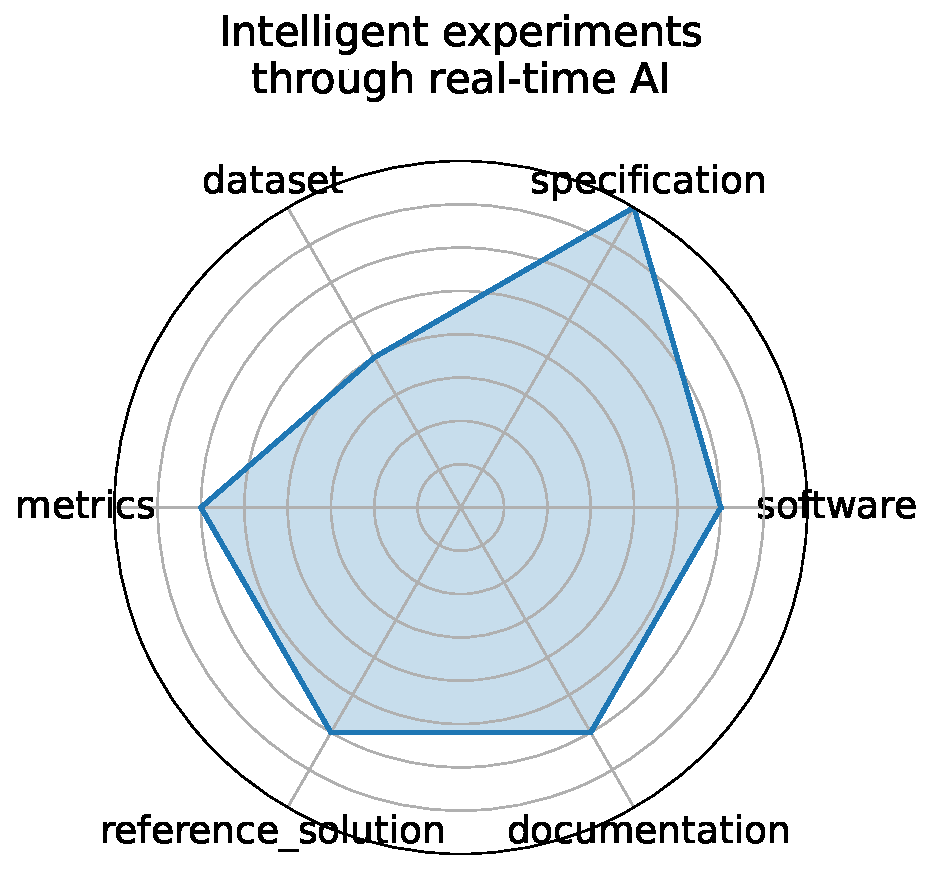
\includegraphics[width=0.2\textwidth]{intelligent_experiments_through_real-time_ai_radar.pdf}
\end{description}
}}
\clearpage